\documentclass{article}

\usepackage[portuguese]{babel}

\usepackage{amsmath, amssymb}
\usepackage{graphicx}
\usepackage{listings}
\usepackage[colorlinks=true, allcolors=blue]{hyperref}

\usepackage[section]{placeins}

\title{Relatório 01}
\author{Vinícius de Oliveira Peixoto Rodrigues (245294)}
\date{Agosto de 2022}

\begin{document}
\maketitle

\section*{Questão 1}

\subsection*{Item (a)}

Foi gerado um arquivo \texttt{teste.a}, e o programa teve a seguinte saída:

\begin{figure}[!ht]
    \begin{center}
        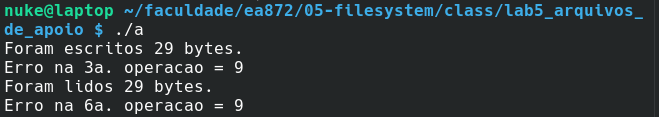
\includegraphics[width=\textwidth]{images/item_a.png}
    \end{center}
\end{figure} 

\subsection*{Item (b)}

Sim; da man entry do \texttt{open}:

\begin{lstlisting}[breaklines]
    creat()
    A call to creat() is equivalent to calling open() with flags equal to O_CREAT|O_WRONLY|O_TRUNC.
\end{lstlisting}

\subsection*{Item (c)}

O argumento \texttt{mode\_t mode} da syscall \texttt{open} serve para definir as permissões a serem dadas para um arquivo se ele for criado a partir da syscall, o que exige que as flags \texttt{O\_CREAT} ou \texttt{O\_TMPFILE} estejam setadas. Do manual:

\begin{lstlisting}[breaklines]
    The mode argument specifies the file mode bits to be
    applied when a new file is created.  If neither O_CREAT
    nor O_TMPFILE is specified in flags, then mode is ignored
    (and can thus be specified as 0, or simply omitted).  The
    mode argument must be supplied if O_CREAT or O_TMPFILE is
    specified in flags; if it is not supplied, some arbitrary
    bytes from the stack will be applied as the file mode. 
\end{lstlisting}

\subsection*{Item (d)}


O erro na 3a operação se deve ao fato de que o \texttt{creat} é equivalente a um \texttt{open(..., O\_CREAT | O\_WRONLY | O\_TRUNC)}, de modo que o descritor \texttt{fd1} está em modo write-only (e não pode ser lido). O erro na 6a operação é porque o descritor \texttt{fd2} foi aberto em modo read-only.

\section*{Questão 2}

\subsection*{Itens (a) e (b)}

\begin{figure}[!ht]
    \begin{center}
        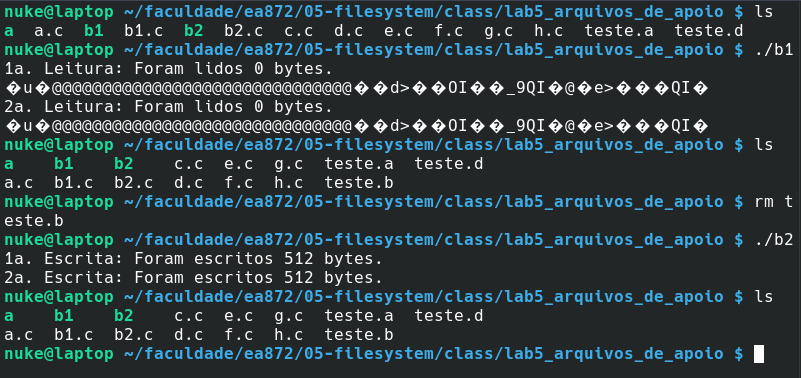
\includegraphics[width=\textwidth]{images/questao_2_ab.png}
    \end{center}
\end{figure} 

Nos dois casos, foi criado um arquivo \texttt{teste.b} (visto que ele foi aberto com \texttt{O\_CREAT}). No programa \texttt{b1}, ele lê lixo (visto que não havia nada escrito no programa ainda). No programa \texttt{b2} ele escreve asteriscos no programa.

\newpage
\subsection*{Item (c)}

\begin{figure}[!ht]
    \begin{center}
        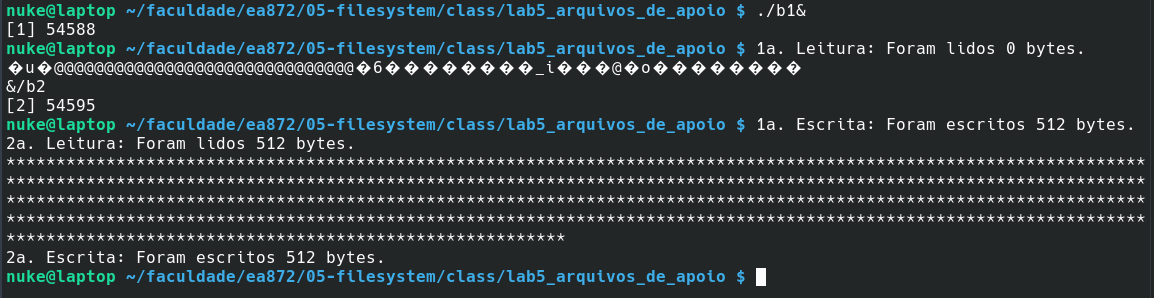
\includegraphics[width=\textwidth]{images/questao_2_c.png}
    \end{center}
\end{figure} 
\FloatBarrier

O programa \texttt{b1} faz uma primeira leitura e lê lixo (não havia nada escrito no arquivo); em seguida, o programa \texttt{b2} escreve no arquivo \texttt{test.b}, e depois o programa \texttt{b1} lê de novo o arquivo, dessa vez lendo os asteriscos recém-escritos.

\newpage
\subsection*{Item (d)}

Isso é possível porque file descriptors são essencialmente só ponteiros para estruturas de dados do kernel; como nós temos apenas um writer e um reader, não há problemas em ter dois processos separados acessando um arquivo. Seria problemático se houvesse mais de um writer com file descriptor obtido por duas chamadas de \texttt{open} diferentes (porque aí o file offset/status dos arquivos não estaria sincronizados, de modo que os dois writers pisariam no pé um do outro).

\newpage
\section*{Questão 3}

\subsection*{Item (a)}

O programa cria um arquivo \texttt{testec1.txt}, escreve a frase \texttt{Este e' o arquivo de teste c1: }; em seguida, move o file offset (que indica o final do arquivo 20031 bytes para frente), e escreve uma mensagem no final (de modo que o arquivo final tem vários KB).

Em seguida, o programa cria um outro arquivo \texttt{testec2.txt}, escreve uma mensagem similar no começo, depois escreve em loop 20 mil caracteres \texttt{\$} e uma mensagem final (de modo que ele também tem vários KB).

\subsection*{Item (b)}

\begin{lstlisting}[breaklines]
    > ls -l testec*
    -rw------- 1 nuke nuke 20059 Sep 21 16:39 testec1.txt
    -rw------- 1 nuke nuke 20059 Sep 21 16:39 testec2.txt

    > ls -s testec*
    8 testec1.txt  20 testec2.txt
\end{lstlisting}

\subsection*{Item (c)}

O sistema operacional tem a liberdade de escolher quantos blocos alocar para cada arquivo; como o arquivo \texttt{testec1.txt} tem um buraco enorme no meio dele (porque nós "aumentamos" o tamanho dele artificialmente usando um \texttt{lseek}), o S.O. só aloca 8 blocos (o tamanho de blocos reportado pelo \texttt{GNU ls} é 1024 bytes, de modo que o tamanho físico alocado é 1024 * 8 = 8 KB). Para o outro arquivo, que é preenchido completamente, o S.O. aloca 20 * 1024 = 20 KB físicos (onde cabe o arquivo inteiro de 20K caracteres).

\end{document}
